\subsection{Ribbon-100L parametric equation}

\begin{table}[ht]
	\begin{center}
		\begin{tabular}[top]{ |p{16.0 cm}| }
			
			\rowcolor{LIGHTCYAN}
			\hline \textbf{No. 10 - Ribbon-100L parametric curve}\\
			
			\begin{eqnarray}
		        t(u) & = & 4(u - 0.50) \nonumber \\
	            x(u) & = & 10t^2 \nonumber \\   
	            y(u) & = & 10t^3 - 30t + 30 \nonumber \\
	            u & \in & [0.0, 1.0] \nonumber
			\end{eqnarray}
			
			
			Open ended curve (10 times larger than RIBBON-10L)\\
			Overall Single loop, smooth convex curves\\
			Reflection x-axis: non-symmetrical\\
			Reflection y-axis: non-symmetrical\\
			\frame{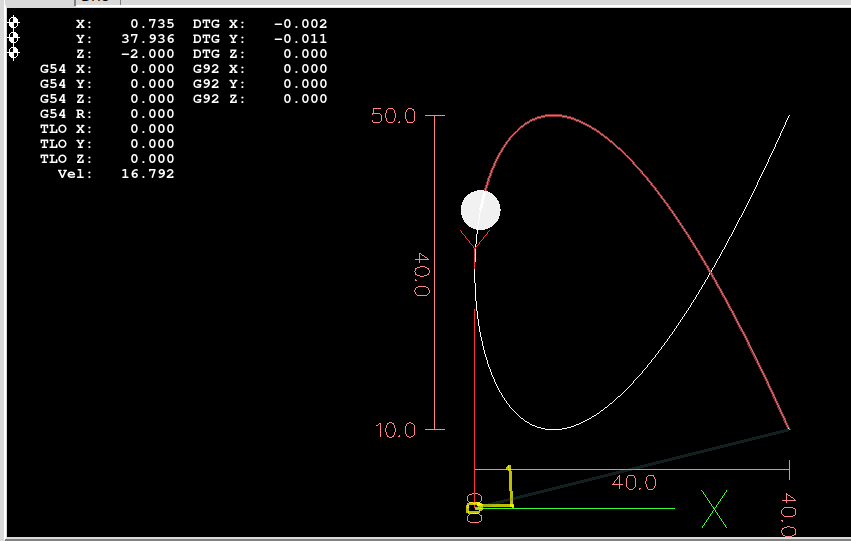
\includegraphics[width=0.575\textwidth]{./07-images/img-Ch5/RIBBON-100L-Axis.png}}
			\frame{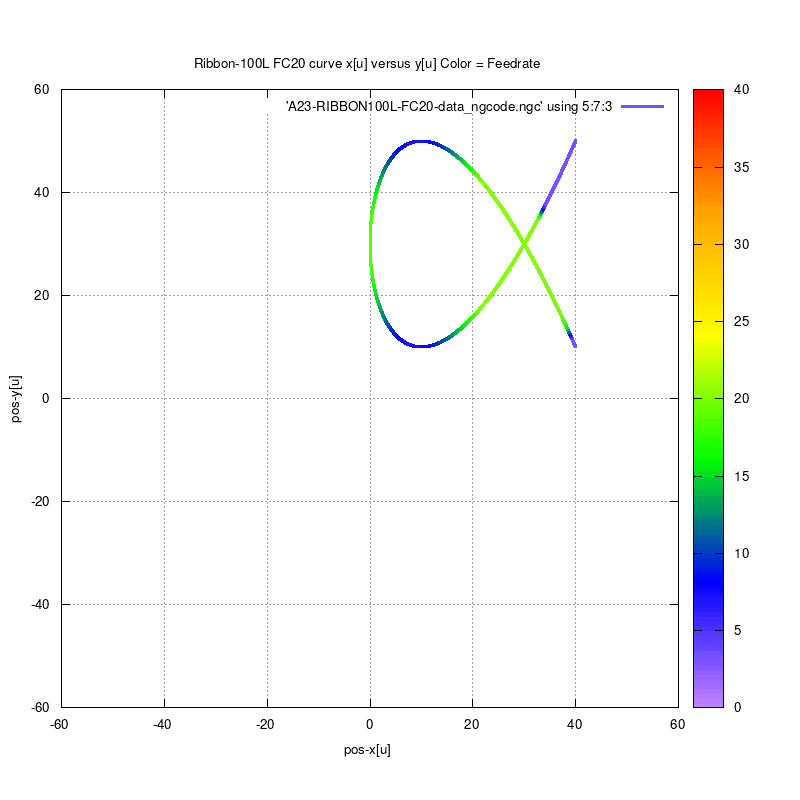
\includegraphics[width=0.370\textwidth]{./07-images/img-Ch5/RIBBON-100L-Feedrate.png}}\\
			
			\hline
		\end{tabular}
		\caption{Ribbon-100L equation and dimensions}
	    \label{table:Ribbon-100L equation and dimensions}
	\end{center}
\end{table}  
